% !TeX program = platex
\documentclass{jarticle}
%数式
\usepackage{amsmath,amssymb} 
%図
\usepackage[dvipdfmx]{graphicx,color} 
\usepackage{adjustbox}
\usepackage{here}
\usepackage{caption} 
\usepackage{subcaption}
\usepackage{cleveref}  
%表
\usepackage{makecell} %セルを定義する
%グラフ
\usepackage{pgfplots}
\pgfplotsset{compat=1.18}
%その他
\usepackage{bm}
\usepackage{url}
\usepackage{siunitx}
\sisetup{inter-unit-product=\ensuremath{{}\cdot{}}} % 単位間に "·" を入れる
\usepackage{cite}
\usepackage{comment}  %\begin{comment} と \end{comment} の間に記述した内容が全て無視される。
                      %\includecomment{comment}でコメントブロック
\usepackage{robomech}

\def\authorinfo{
    \begin{tabular}{ll}
		○\hspace{1zw}小森文雄 (京都大)
        \hspace{1zw}正　川節 拓実 (京都大)\\
        \hspace{1zw}正　細田 耕 (京都大) 
    \end{tabular}
    \smallskip \\  % 適切な間隔
    \begin{tabular}{l}
        {\small FUMIO KOMORI, Kyoto University, komori.fumio.87e@st.kyoto-u.ac.jp}\\
        {\small Takumi KAWASETSU, Kyoto University}\\
        {\small Koh HOSODA, Kyoto University}
    \end{tabular}
}

\begin{document}
\makeatletter
\title{触覚とソフトフィンガーを用いた模倣学習による柔軟シートのマニピュレーション
}
{Flexible Sheet Manipulation through Imitation Learning with Tactile Sensing and Soft Robotic Fingers}

\author{\authorinfo}
\makeatother

\abstract{% !TeX root = ../main.tex
This paper presents a method for integrating tactile information from soft robotic fingers into imitation learning for robotic manipulation tasks. The proposed system utilizes simple ion liquid sensors embedded in soft fingers to capture tactile feedback, which is then directly fed into a learning model based on Action Chunking with Transformers (ACT). The method is evaluated on a sheet-like flexible object grasping task that involves visual occlusion, demonstrating that the integration of tactile information enables robust performance even with simple sensors. The results suggest that the combination of soft robotic fingers and learning-based approaches can effectively handle complex contact transitions and environmental variations in manipulation tasks.
\small 
}

\keywords{imitation learning, tactile sensing, soft robotic fingers,flexible object manipulation}

\maketitle
\thispagestyle{empty}
\pagestyle{empty}

\maintext

\section{緒言}%===========================
ロボットの模倣学習において，視覚的な遮蔽や柔軟物の変形を伴うタスクの遂行には，視覚情報だけでなく触覚情報の活用が不可欠であるが，その触覚情報として従来の高精度な力覚センサ等を用いると，コストがかかり，システムも複雑になる\cite{example}．
本報告では，単純な構造を持つイオン液体センサを触覚とするソフトフィンガーを用い，その低次元な変形情報を模倣学習に統合する手法を提案する．また，7自由度ロボットアームを用いた繊細な接触動作の教示データ収集を容易にするため，重力補償を導入したテレオペレーションシステムを構築し，学習と検証を行った．提案手法の評価として，視覚的遮蔽を伴うシート状柔軟物把持タスクを対象に実験を行った．その結果，触覚情報を統合したモデルは高い成功率を示し，単純なセンサであっても環境変動に対してロバストな動作生成ができることが示された．


\section{触覚とソフトフィンガーを備えた7自由度ロボットアームの模倣学習}
% !TeX root = ../main.tex
\begin{figure}[htbp]
  \centering
  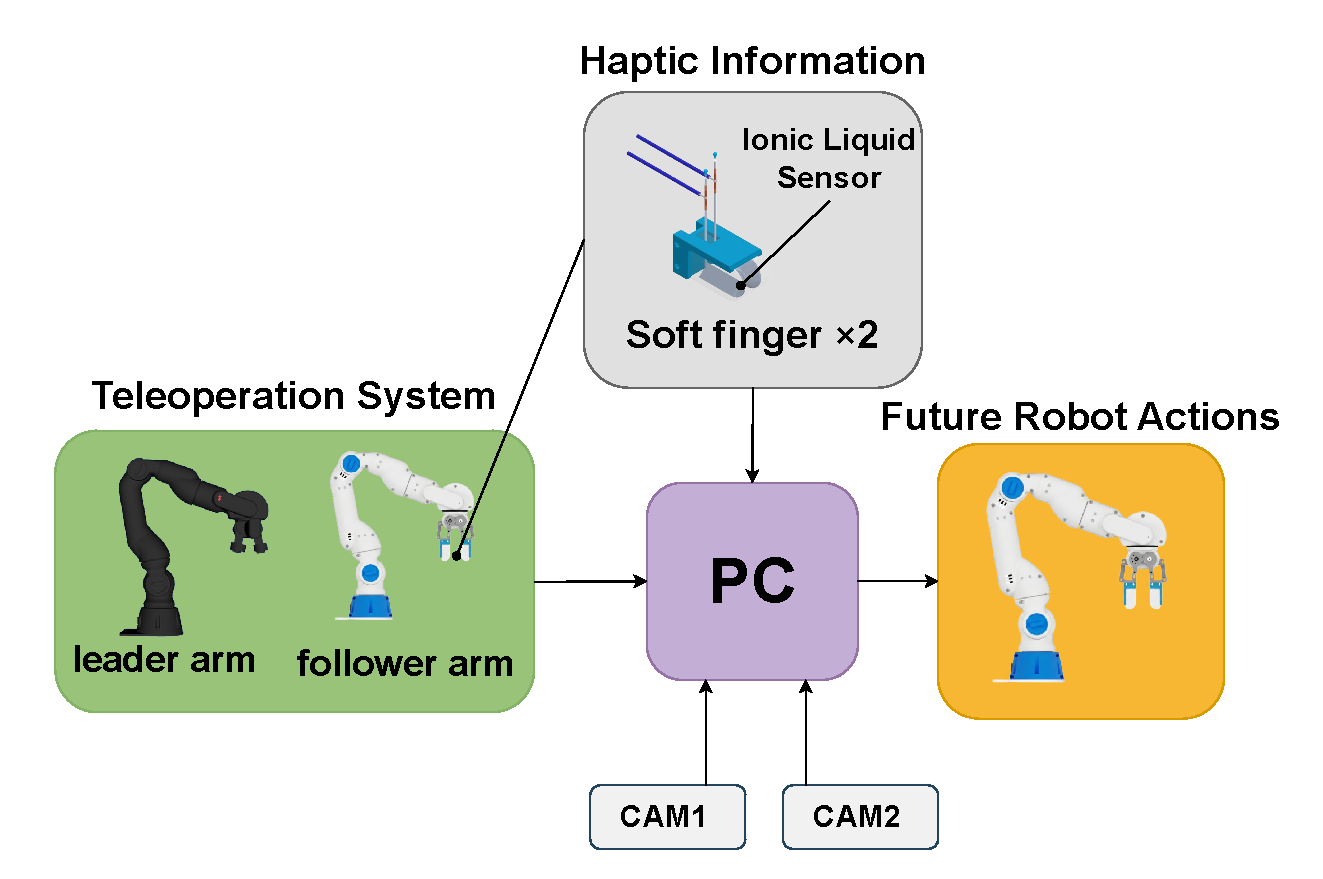
\includegraphics[width=0.95\linewidth]{tex/Image/imitationlearningsystemrobomech.drawio.pdf}
  \caption{Overview of the proposed imitation learning system using a teleoperation setup and haptic information}
  \label{fig:robot_system}
\end{figure}
% 本章では，提案する模倣学習手法について述べる．Fig\ref{fig:robot_system}にシステムの構成図を示す．
本システムは，リーダー・フォロワー構成のロボットアーム，フォロワーアーム先端に2つのイオン液体センサを内蔵したソフトフィンガー，フォロワーアームを側面・上面から観測するRGBカメラ2台，および制御・学習用PCで構成される．教示データ収集時は操作者がリーダーアームを操作し，フォロワーアームで物体操作を行う．収集データを用いてフォロワーアームの動作モデルを模倣学習し，入力にはカメラ画像，関節角度，ソフトフィンガーの触覚情報を用いる．学習後は，フォロワーアームが自律的に物体操作タスクを実行する．\par

まず，ハードウェア構成を述べる．本研究では，リーダー・フォロワー方式のテレオペレーションシステムとして，RT社製7自由度ロボットアームCRANE-X7を2台使用する．アーム7自由度とグリッパ1自由度を備え，全体で8自由度である．1台をリーダー，もう1台をフォロワーとして用い，フォロワーのグリッパにソフトフィンガーを取り付けている．\par
このフィンガーはシリコンゴム本体とPLA製の爪部からなり，内部にイオン液体を封入した流路を持つ触覚センサを埋め込んでいる．イオン液体は導電性に加え，不揮発性，難燃性，高い熱安定性を有する\cite{armandIonicliquidMaterialsElectrochemical2009}．対象物との接触で流路が変形すると，断面積 $A$ と長さ $L$ が変化する．
この幾何学的変化は，イオン液体固有の電気抵抗率 $\rho$ を用いて，抵抗値 $R$ が次式
\begin{equation}
  R = \rho \frac{L}{A}
\end{equation}
で表されるため，検出できる\cite{chossatSoftStrainSensor2013}．フォロワーアームには平行リンク機構を用いた2指平行グリッパを取り付け，2つのソフトフィンガーからセンサ情報を取得する．\par
% \begin{figure}[htbp]
%   \centering
%   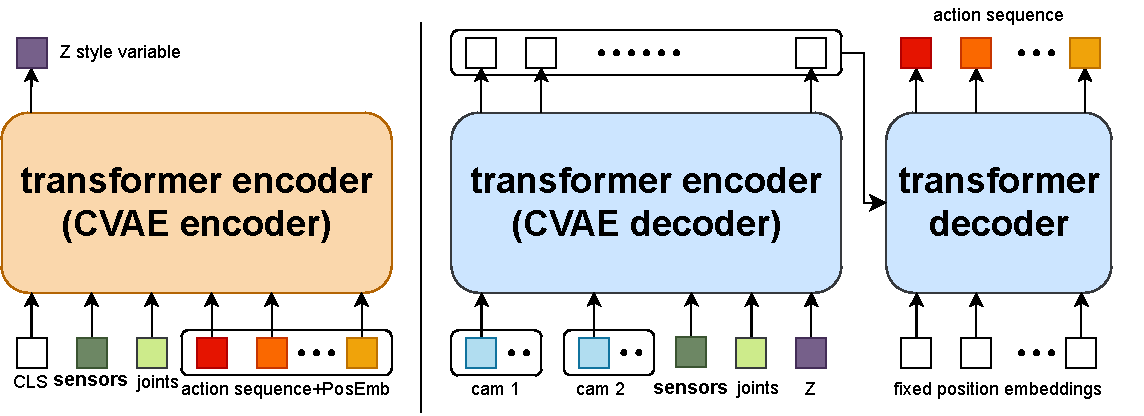
\includegraphics[width=1.1\linewidth]{tex/Image/ACT.drawio.pdf}
%   \caption{Action Chunking with Transformers (ACT) architecture used for imitation learning．This model extends the conventional ACT framework by introducing distinct sensor embeddings．}
%   \label{fig:act}
% \end{figure}
本研究では，接触を伴う複雑タスクを7自由度ロボットアームで学習するため，Action Chunking with Transformers (ACT) \cite{zhaoLearningFineGrainedBimanual2023}を採用する．ACTはConditional Variational Autoencoder (CVAE)とTransformerを組み合わせたモデルで，現在の観測から未来数ステップのアクション系列（Action Chunk）を一括予測することで，時系列の長期依存を学習し，滑らかな動作生成を実現する．本アーキテクチャの特徴は，従来のACTにセンサ値を新たなモダリティとして追加した点である．関節角度と同様にセンサ値をトークン化し，CVAEエンコーダーとデコーダーに画像特徴量・関節情報と並列入力することで，触覚を統合した動作生成を可能にした．実装には，Hugging Faceが提供する模倣学習ライブラリlerobot\cite{cadene2024lerobot}を用いた．\par
リーダーアーム操作時は，CRANE-X7の重量負担を軽減するため重力補償制御を適用する．現在の関節位置から各関節に作用する重力トルクを計算し，逆方向のトルクを各関節に加えてアーム重量を相殺することで，操作者は質量感を抑えた直感的な教示動作を行える．
% lerobotはデータ収集から学習，評価までを統一的に扱える優れたフレームワークであるが，重力補償機能はPython実装では制御周期の安定性やリアルタイム性に課題があった．そこで本研究では，RT社の提供するCRANE-X7の重力補償のC++ライブラリをpybind11を用いてlerobotのPython環境に組み込む実装を行った．これにより，最新の学習フレームワークの恩恵を受けつつ，C++による滑らかで高応答な重力補償制御を両立させている．

\section{シート状柔軟物のつまみ上げ実験}
% !TeX root = ../main.tex
\begin{figure}[htbp]
  \centering
  \begin{minipage}[t]{0.70\linewidth}
    \vspace{0pt}
    \centering
    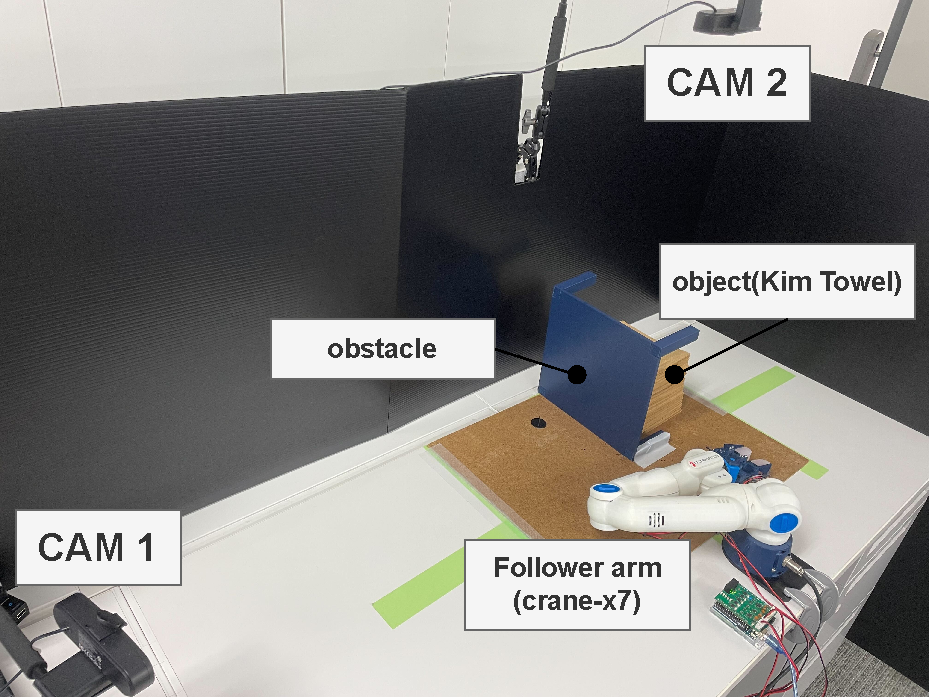
\includegraphics[width=\linewidth]{tex/Image/experimentsetup.drawio.pdf}
  \end{minipage}\hfill
  \begin{minipage}[t]{0.30\linewidth}
    \vspace{0pt}
    \centering
    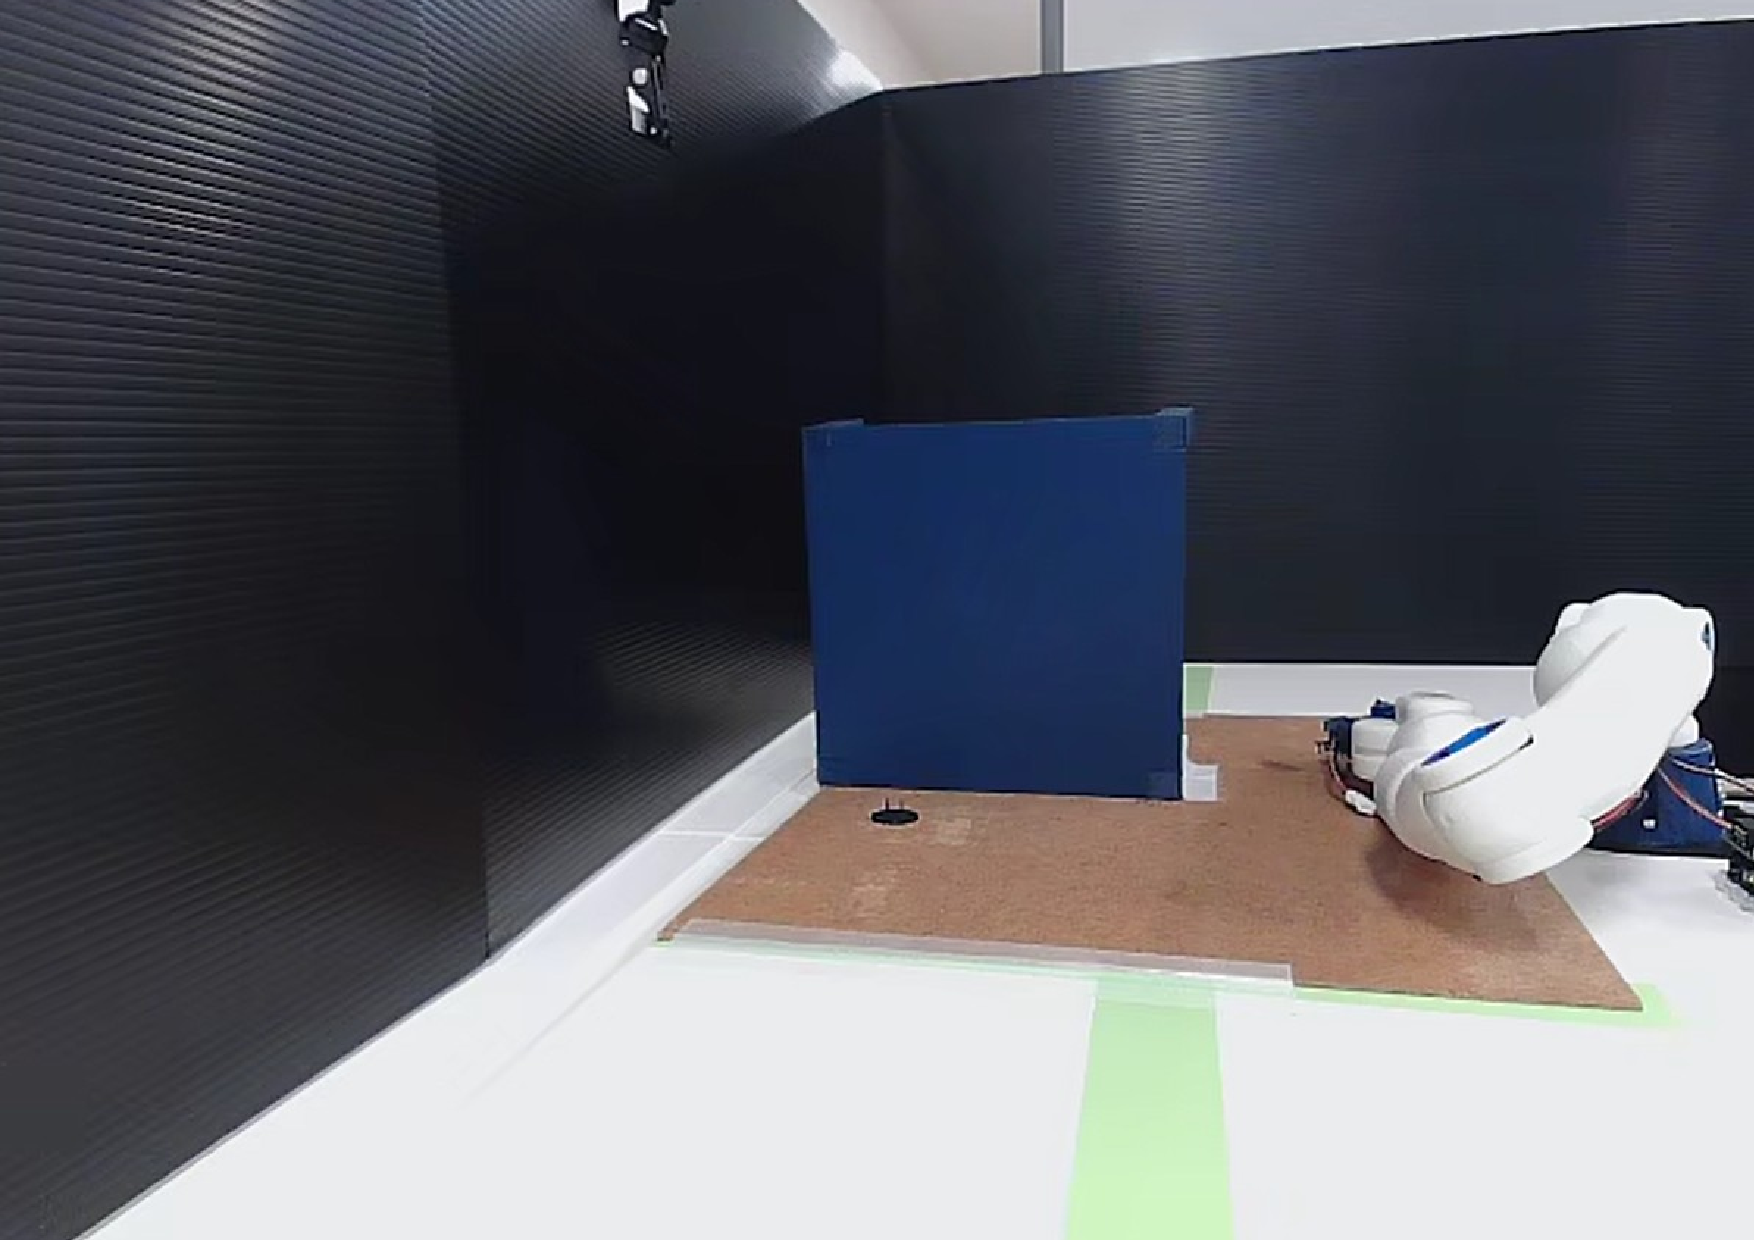
\includegraphics[width=\linewidth]{tex/Image/lateralview.pdf}
    {\footnotesize CAM1\par}
    \vspace{0.5mm}
    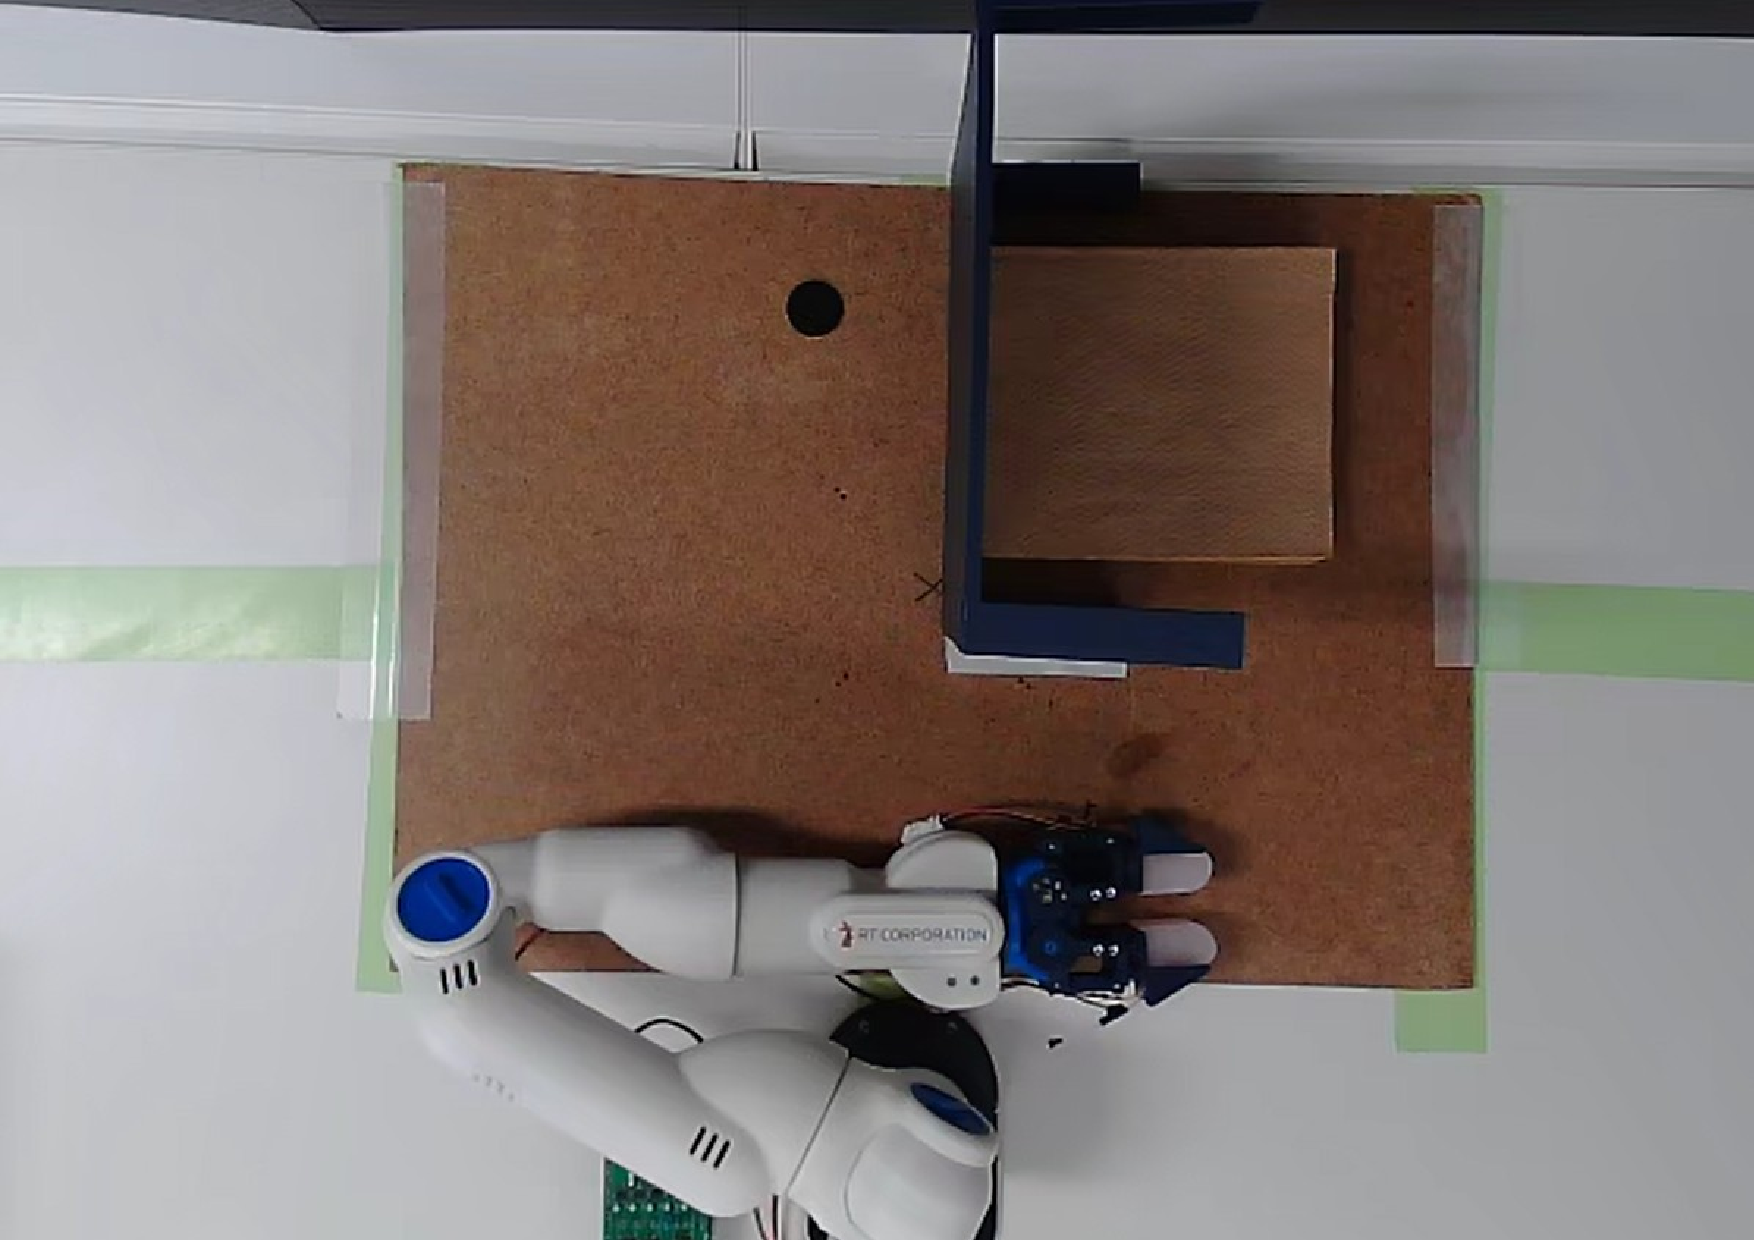
\includegraphics[width=\linewidth]{tex/Image/topview.pdf}
    {\footnotesize CAM2\par}
  \end{minipage}
  \caption{Experimental setup and camera views. The obstacle occludes the Kim towel in Camera 1 (lateral), while Camera 2 provides the top view.}
  \label{fig:experiment_setup_grasp}
\end{figure}
\vspace{-1.0ex}
本実験では，触覚情報の有用性を検証するため，触覚センサ情報の有無（sensor\_on / sensor\_off）によるタスク成功率を比較した．タスクは，積層キムタオルを把持して所定位置へ搬送する動作とした．また，双腕協調作業や深箱内操作で生じる視覚遮蔽を再現するため，Fig.~\ref{fig:experiment_setup_grasp}のように中央に障害物を設置し，側面カメラ（Camera 1）から対象物（キムタオル）の高さ情報が得られない環境を構築した．\par

教示データは，Fig.~\ref{fig:experiment_setup_grasp}のセットアップでリーダーアームをテレオペレーションし，積層キムタオルの最上位1枚を把持して障害物左側へ搬送する動作から収集した．積層枚数は50，40，30，20，10枚の5条件とし，各条件2回，計10回分を収集した．収集時には触覚センサの生データ値も記録し，学習ではセンサ値を使用しない条件（sensor\_off）と使用する条件（sensor\_on）の2条件でモデルを生成した．学習モデルのトレーニングは，AMD Ryzen 9 9950X CPU，NVIDIA GeForce RTX 5080 GPU (16GB)，メモリ64GBを搭載したPC（OS: Ubuntu 24.04.3 LTS）で実施した．ハイパーパラメータは，バッチサイズ8，学習ステップ数20,000に設定した．学習時間はいずれも約40分であった．\par

続いて，タスクの評価方法と成功率を示す．タスクの成功条件は，「積層キムタオルから1枚のみを把持し，障害物左側の目標領域へ搬送すること」と定義した．目標領域は障害物左側全域である．最初の把持動作でキムタオルを掴み損ね，ロボットが自律的に再把持（リトライ）した場合は，以降の動作にかかわらず失敗と判定した．以下に各条件での成功率を示す．教示時にはない1枚と60枚の場合を加えて，それぞれ5回の試行を行いその成功率を算出した．
% Table\ref{tab:success_rate_30mm}は指先を教示データと同じ長さにした場合，Table\ref{tab:success_rate_0mm}は指先を30mm短くした場合の成功率である．\par

\definecolor{sensoroncolor}{gray}{0.20}
\definecolor{sensoroffcolor}{gray}{0.75}

\begin{figure}[htbp]
  \centering
  \begin{tikzpicture}
    \begin{axis}[
      ybar,
      bar width=7pt,
      xlabel={Number of Sheets},
      ylabel={Success Rate (\%)},
      xtick=data,
      symbolic x coords={1,10,20,30,40,50,60},
      ymin=0, ymax=110,
      ytick={0,20,...,100},
      ymajorgrids=true,
      grid style={dashed, gray!50},
      legend style={at={(1.02,1)}, anchor=north west, font=\small},
      width=0.70\linewidth,
      height=0.48\linewidth,
    ]
    \addplot[fill=sensoroncolor, draw=black] coordinates {
      (1,100) (10,100) (20,100) (30,100) (40,100) (50,100) (60,100)
    };
    \addlegendentry{With sensor}
    \addplot[fill=sensoroffcolor, draw=black] coordinates {
      (1,20) (10,100) (20,100) (30,100) (40,0) (50,60) (60,20)
    };
    \addlegendentry{Without sensor}
    \end{axis}
  \end{tikzpicture}
  \caption{Success rates with and without tactile sensing.}
  \label{fig:success_rate}
\end{figure}
\vspace{-1.0ex}

sensor\_on条件は教示データに含まれない高さ条件でも成功率100\%を達成した．一方，sensor\_off条件では，把持高さが教示データと異なる場合に成功率が著しく低下し，同一高さでも一部で低下が見られた．これは，ソフトフィンガー接触時の抵抗値変化をトリガーに把持動作が調整された，すなわち，触覚情報が視覚情報の不確実性を補完したと示唆される．
sensor\_off条件の失敗エピソードでは，アームが対象手前で停止する，あるいは押し込みながらつかみ損ねる動作が見られた．このことから，失敗は画像特徴量による高さ推定精度の不足に起因すると考えられる．
% また，指の長さが教示時より短い場合でも，sensor\_on条件は概ね高い成功率を維持した．ただし，対象物が1枚の場合は把持に失敗し，成功率は0\%となった．\par

% \section{議論} 
% % !TeX root = ../main.tex
教示時と同じ指のSensor\_off条件において成功率の低下およびばらつきが生じた主要因として，視覚情報のみに依存した高さ推定の限界が挙げられる．本実験環境では，側面カメラは障害物によるオクルージョンが発生し，上面カメラは深度情報を持たないRGBカメラである．そのため，積層されたキムタオルの高さ変化を画像特徴の変化としてのみ捉える必要があるが，照明条件の変動やわずかな位置ずれにより，その特徴量は不安定となる．成功しているエピソードに関しては，上面カメラが対象物の影等を捉えて画像特徴による高さ推定が成功したか，指の柔軟性が推定誤差を吸収した結果であると推察される．\par
教示時より短い指のSensor\_on条件において1枚の把持が失敗した原因は，教示データに含まれる関節角度の分布にあると考えられる．教示データには，指が短くなった分だけアームを深く下ろすような動作データは含まれていない．本手法で用いたACTアーキテクチャは，触覚情報を利用することで接触時の微調整は可能であるが，教示された関節角度の分布から大きく逸脱するような大域的な軌道修正（教示時よりもさらに深くアームを下げる動作）までは生成できない．したがって，1枚の条件での失敗は，学習ベースの手法における汎化性能の限界を示していると言える．\par
教示時より短い指のSensor\_off条件において30枚以上の高さで高い成功率を示したのは，教示データと同一の指長さでは画像特徴量による高さ推定のずれで深く掴みに行き過ぎてつかむことが難しくなっていたが，指が短くなったことでそのずれを吸収し適切な深さになったためと考えられる． 

\section{結言}
提案手法は視覚情報のみでは把握困難な環境変動に対しても，接触時のセンサ応答に基づき把持動作を適応的に調整可能であることを示した．特筆すべきは，用いた触覚情報が抵抗値変化という低次元かつ物理的な意味が一意に定まらないデータであったにもかかわらず，模倣学習によって視覚情報や動作文脈と適切に統合され，タスク遂行に必要な接触検知や動作トリガーとして機能した点である．この結果は，高価な力覚センサによる明示的な状態推定を行わずとも，単純なセンサと学習モデルの組み合わせにより，実環境の不確実性に対してロバストな適応が可能であることを実証するものである．\par

一方で，獲得された方策の汎化能力は教示データの運動学的範囲に依存しており，教示時の可動域を大きく逸脱するような幾何学的制約に対しては，触覚情報の活用のみでは補正しきれない限界も確認された．これは，学習ベースの手法における分布外データへの対応という課題を改めて浮き彫りにするものである．

% !TeX root = ../main.tex
\acknowledgment
本研究は，JST戦略的創造研究推進事業CREST JPMJCR2555の助成を受けたものである．


\footnotesize
\begin{thebibliography}{99}
% !TeX root = ../main.tex
\bibitem{zhaoLearningFineGrainedBimanual2023}
Zhao, T. Z., Kumar, V., Levine, S. and Finn, C.,
``Learning fine-grained bimanual manipulation with low-cost hardware,''
arXiv:2304.13705, 2023.

\bibitem{zhuDeformableFragileObject2025}
Zhu, Y., Yang, D. and Lee, Y.,
``Deformable and fragile object manipulation: A review and prospects,''
{\it Sensors}, vol.25, no.17, 2025.

\bibitem{kadiDataDrivenRoboticManipulation2023}
Kadi, H. A. and Terzic, K.,
``Data-driven robotic manipulation of cloth-like deformable objects: The present, challenges and future prospects,''
{\it Sensors}, vol.23, no.5, article 2389, 2023.

\bibitem{example}
Chi, C., Sun, X., Xue, N., Li, T. and Liu, C.,
``Recent progress in technologies for tactile sensors,''
{\it Sensors}, vol.18, no.4, article 948, 2018.

\bibitem{armandIonicliquidMaterialsElectrochemical2009}
Armand, M., Endres, F., MacFarlane, D. R., Ohno, H. and Scrosati, B.,
``Ionic-liquid materials for the electrochemical challenges of the future,''
{\it Nature Materials}, vol.8, no.8, pp.621--629, 2009.

\bibitem{chossatSoftStrainSensor2013}
Chossat, J.-B., Park, Y.-L., Wood, R. J. and Duchaine, V.,
``A soft strain sensor based on ionic and metal liquids,''
{\it IEEE Sensors Journal}, vol.13, no.9, pp.3405--3414, 2013.

\bibitem{cadene2024lerobot}
Cadene, R. and et al.,
``LeRobot: state-of-the-art machine learning for real-world robotics in PyTorch,''
GitHub repository, 2024.

\end{thebibliography}
\normalsize
\end{document}
